\documentclass[twoside]{book}

% Packages required by doxygen
\usepackage{fixltx2e}
\usepackage{calc}
\usepackage{doxygen}
\usepackage[export]{adjustbox} % also loads graphicx
\usepackage{graphicx}
\usepackage[utf8]{inputenc}
\usepackage{makeidx}
\usepackage{multicol}
\usepackage{multirow}
\PassOptionsToPackage{warn}{textcomp}
\usepackage{textcomp}
\usepackage[nointegrals]{wasysym}
\usepackage[table]{xcolor}

% NLS support packages
\usepackage[spanish]{babel}
% Font selection
\usepackage[T1]{fontenc}
\usepackage[scaled=.90]{helvet}
\usepackage{courier}
\usepackage{amssymb}
\usepackage{sectsty}
\renewcommand{\familydefault}{\sfdefault}
\allsectionsfont{%
  \fontseries{bc}\selectfont%
  \color{darkgray}%
}
\renewcommand{\DoxyLabelFont}{%
  \fontseries{bc}\selectfont%
  \color{darkgray}%
}
\newcommand{\+}{\discretionary{\mbox{\scriptsize$\hookleftarrow$}}{}{}}

% Page & text layout
\usepackage{geometry}
\geometry{%
  a4paper,%
  top=2.5cm,%
  bottom=2.5cm,%
  left=2.5cm,%
  right=2.5cm%
}
\tolerance=750
\hfuzz=15pt
\hbadness=750
\setlength{\emergencystretch}{15pt}
\setlength{\parindent}{0cm}
\setlength{\parskip}{3ex plus 2ex minus 2ex}
\makeatletter
\renewcommand{\paragraph}{%
  \@startsection{paragraph}{4}{0ex}{-1.0ex}{1.0ex}{%
    \normalfont\normalsize\bfseries\SS@parafont%
  }%
}
\renewcommand{\subparagraph}{%
  \@startsection{subparagraph}{5}{0ex}{-1.0ex}{1.0ex}{%
    \normalfont\normalsize\bfseries\SS@subparafont%
  }%
}
\makeatother

% Headers & footers
\usepackage{fancyhdr}
\pagestyle{fancyplain}
\fancyhead[LE]{\fancyplain{}{\bfseries\thepage}}
\fancyhead[CE]{\fancyplain{}{}}
\fancyhead[RE]{\fancyplain{}{\bfseries\leftmark}}
\fancyhead[LO]{\fancyplain{}{\bfseries\rightmark}}
\fancyhead[CO]{\fancyplain{}{}}
\fancyhead[RO]{\fancyplain{}{\bfseries\thepage}}
\fancyfoot[LE]{\fancyplain{}{}}
\fancyfoot[CE]{\fancyplain{}{}}
\fancyfoot[RE]{\fancyplain{}{\bfseries\scriptsize Generado por Doxygen }}
\fancyfoot[LO]{\fancyplain{}{\bfseries\scriptsize Generado por Doxygen }}
\fancyfoot[CO]{\fancyplain{}{}}
\fancyfoot[RO]{\fancyplain{}{}}
\renewcommand{\footrulewidth}{0.4pt}
\renewcommand{\chaptermark}[1]{%
  \markboth{#1}{}%
}
\renewcommand{\sectionmark}[1]{%
  \markright{\thesection\ #1}%
}

% Indices & bibliography
\usepackage{natbib}
\usepackage[titles]{tocloft}
\setcounter{tocdepth}{3}
\setcounter{secnumdepth}{5}
\makeindex

% Hyperlinks (required, but should be loaded last)
\usepackage{ifpdf}
\ifpdf
  \usepackage[pdftex,pagebackref=true]{hyperref}
\else
  \usepackage[ps2pdf,pagebackref=true]{hyperref}
\fi
\hypersetup{%
  colorlinks=true,%
  linkcolor=blue,%
  citecolor=blue,%
  unicode%
}

% Custom commands
\newcommand{\clearemptydoublepage}{%
  \newpage{\pagestyle{empty}\cleardoublepage}%
}

\usepackage{caption}
\captionsetup{labelsep=space,justification=centering,font={bf},singlelinecheck=off,skip=4pt,position=top}

%===== C O N T E N T S =====

\begin{document}

% Titlepage & ToC
\hypersetup{pageanchor=false,
             bookmarksnumbered=true,
             pdfencoding=unicode
            }
\pagenumbering{alph}
\begin{titlepage}
\vspace*{7cm}
\begin{center}%
{\Large Box2D \\[1ex]\large 1.\+0 }\\
\vspace*{1cm}
{\large Generado por Doxygen 1.8.14}\\
\end{center}
\end{titlepage}
\clearemptydoublepage
\pagenumbering{roman}
\tableofcontents
\clearemptydoublepage
\pagenumbering{arabic}
\hypersetup{pageanchor=true}

%--- Begin generated contents ---
\chapter{Indice de namespaces}
\section{Lista de \textquotesingle{}namespaces\textquotesingle{}}
Lista de los \textquotesingle{}namespaces\textquotesingle{}, con una breve descripción\+:\begin{DoxyCompactList}
\item\contentsline{section}{\mbox{\hyperlink{namespacephysics}{physics}} }{\pageref{namespacephysics}}{}
\end{DoxyCompactList}

\chapter{Indice jerárquico}
\section{Jerarquía de la clase}
Esta lista de herencias esta ordenada aproximadamente por orden alfabético\+:\begin{DoxyCompactList}
\item b2\+Contact\+Listener\begin{DoxyCompactList}
\item \contentsline{section}{physics\+:\+:Collison}{\pageref{classphysics_1_1_collison}}{}
\end{DoxyCompactList}
\item \contentsline{section}{physics\+:\+:Box2\+D\+Object}{\pageref{classphysics_1_1_box2_d_object}}{}
\item \contentsline{section}{Box2\+D\+Object}{\pageref{class_box2_d_object}}{}
\item \contentsline{section}{Circle\+Particle}{\pageref{class_circle_particle}}{}
\item \contentsline{section}{Collision}{\pageref{class_collision}}{}
\item \contentsline{section}{physics\+:\+:Particle}{\pageref{classphysics_1_1_particle}}{}
\begin{DoxyCompactList}
\item \contentsline{section}{physics\+:\+:Circle\+Particle}{\pageref{classphysics_1_1_circle_particle}}{}
\end{DoxyCompactList}
\item \contentsline{section}{Particle}{\pageref{class_particle}}{}
\item \contentsline{section}{physics\+:\+:Particle\+System$<$ P\+A\+R\+T\+I\+C\+LE $>$}{\pageref{classphysics_1_1_particle_system}}{}
\item \contentsline{section}{Particle\+System}{\pageref{class_particle_system}}{}
\item \contentsline{section}{physics\+:\+:Particle\+System$<$ Circle\+Particle $>$}{\pageref{classphysics_1_1_particle_system}}{}
\item \contentsline{section}{physics\+:\+:Scene}{\pageref{classphysics_1_1_scene}}{}
\item \contentsline{section}{Scene}{\pageref{class_scene}}{}
\end{DoxyCompactList}

\chapter{Índice de clases}
\section{Lista de clases}
Lista de las clases, estructuras, uniones e interfaces con una breve descripción\+:\begin{DoxyCompactList}
\item\contentsline{section}{\mbox{\hyperlink{classphysics_1_1_box2_d_object}{physics\+::\+Box2\+D\+Object}} }{\pageref{classphysics_1_1_box2_d_object}}{}
\item\contentsline{section}{\mbox{\hyperlink{class_box2_d_object}{Box2\+D\+Object}} \\*Clase en donde se construye y renderiza el objeto Box2D combinado con el objeto S\+F\+ML, para proporcionarle un color }{\pageref{class_box2_d_object}}{}
\item\contentsline{section}{\mbox{\hyperlink{classphysics_1_1_circle_particle}{physics\+::\+Circle\+Particle}} }{\pageref{classphysics_1_1_circle_particle}}{}
\item\contentsline{section}{\mbox{\hyperlink{class_circle_particle}{Circle\+Particle}} \\*Clase en donde se renderizan y updatean las part�cular con forma redondeada, hereda de la clase \char`\"{}\+Particle\char`\"{} }{\pageref{class_circle_particle}}{}
\item\contentsline{section}{\mbox{\hyperlink{class_collision}{Collision}} \\*Clase en donde se llaman a las colisiones de los objetos con otros }{\pageref{class_collision}}{}
\item\contentsline{section}{\mbox{\hyperlink{classphysics_1_1_collison}{physics\+::\+Collison}} }{\pageref{classphysics_1_1_collison}}{}
\item\contentsline{section}{\mbox{\hyperlink{classphysics_1_1_particle}{physics\+::\+Particle}} }{\pageref{classphysics_1_1_particle}}{}
\item\contentsline{section}{\mbox{\hyperlink{class_particle}{Particle}} \\*Clase abstracta en donde se definen m�todos y variables de una part�cula }{\pageref{class_particle}}{}
\item\contentsline{section}{\mbox{\hyperlink{classphysics_1_1_particle_system}{physics\+::\+Particle\+System$<$ P\+A\+R\+T\+I\+C\+L\+E $>$}} }{\pageref{classphysics_1_1_particle_system}}{}
\item\contentsline{section}{\mbox{\hyperlink{class_particle_system}{Particle\+System}} \\*Clase que se encarga de montar el sistema de part�culas, renderizarlo y updatearlo }{\pageref{class_particle_system}}{}
\item\contentsline{section}{\mbox{\hyperlink{classphysics_1_1_scene}{physics\+::\+Scene}} }{\pageref{classphysics_1_1_scene}}{}
\item\contentsline{section}{\mbox{\hyperlink{class_scene}{Scene}} \\*Clase que se encarga de montar la escena, renderizarla y updatearla }{\pageref{class_scene}}{}
\end{DoxyCompactList}

\chapter{Indice de archivos}
\section{Lista de archivos}
Lista de todos los archivos con descripciones breves\+:\begin{DoxyCompactList}
\item\contentsline{section}{\mbox{\hyperlink{_box2_d_object_8cpp}{Box2\+D\+Object.\+cpp}} }{\pageref{_box2_d_object_8cpp}}{}
\item\contentsline{section}{\mbox{\hyperlink{_box2_d_object_8hpp}{Box2\+D\+Object.\+hpp}} }{\pageref{_box2_d_object_8hpp}}{}
\item\contentsline{section}{\mbox{\hyperlink{_circle_particle_8cpp}{Circle\+Particle.\+cpp}} }{\pageref{_circle_particle_8cpp}}{}
\item\contentsline{section}{\mbox{\hyperlink{_circle_particle_8hpp}{Circle\+Particle.\+hpp}} }{\pageref{_circle_particle_8hpp}}{}
\item\contentsline{section}{\mbox{\hyperlink{_collision_8hpp}{Collision.\+hpp}} }{\pageref{_collision_8hpp}}{}
\item\contentsline{section}{\mbox{\hyperlink{main_8cpp}{main.\+cpp}} }{\pageref{main_8cpp}}{}
\item\contentsline{section}{\mbox{\hyperlink{_particle_8hpp}{Particle.\+hpp}} }{\pageref{_particle_8hpp}}{}
\item\contentsline{section}{\mbox{\hyperlink{_particle_system_8hpp}{Particle\+System.\+hpp}} }{\pageref{_particle_system_8hpp}}{}
\item\contentsline{section}{\mbox{\hyperlink{_scene_8cpp}{Scene.\+cpp}} }{\pageref{_scene_8cpp}}{}
\item\contentsline{section}{\mbox{\hyperlink{_scene_8hpp}{Scene.\+hpp}} }{\pageref{_scene_8hpp}}{}
\end{DoxyCompactList}

\chapter{Documentación de namespaces}
\hypertarget{namespacephysics}{}\section{Referencia del Namespace physics}
\label{namespacephysics}\index{physics@{physics}}
\subsection*{Clases}
\begin{DoxyCompactItemize}
\item 
class \mbox{\hyperlink{classphysics_1_1_box2_d_object}{Box2\+D\+Object}}
\item 
class \mbox{\hyperlink{classphysics_1_1_circle_particle}{Circle\+Particle}}
\item 
class \mbox{\hyperlink{classphysics_1_1_collison}{Collison}}
\item 
class \mbox{\hyperlink{classphysics_1_1_particle}{Particle}}
\item 
class \mbox{\hyperlink{classphysics_1_1_particle_system}{Particle\+System}}
\item 
class \mbox{\hyperlink{classphysics_1_1_scene}{Scene}}
\end{DoxyCompactItemize}
\subsection*{typedefs}
\begin{DoxyCompactItemize}
\item 
typedef \mbox{\hyperlink{classphysics_1_1_particle_system}{Particle\+System}}$<$ \mbox{\hyperlink{classphysics_1_1_circle_particle}{Circle\+Particle}} $>$ \mbox{\hyperlink{namespacephysics_a962adae29e6ee31067fabcf90eb01dac}{Circle\+Particle\+System}}
\end{DoxyCompactItemize}


\subsection{Documentación de los \textquotesingle{}typedefs\textquotesingle{}}
\mbox{\Hypertarget{namespacephysics_a962adae29e6ee31067fabcf90eb01dac}\label{namespacephysics_a962adae29e6ee31067fabcf90eb01dac}} 
\index{physics@{physics}!Circle\+Particle\+System@{Circle\+Particle\+System}}
\index{Circle\+Particle\+System@{Circle\+Particle\+System}!physics@{physics}}
\subsubsection{\texorpdfstring{Circle\+Particle\+System}{CircleParticleSystem}}
{\footnotesize\ttfamily typedef \mbox{\hyperlink{classphysics_1_1_particle_system}{Particle\+System}}$<$\mbox{\hyperlink{classphysics_1_1_circle_particle}{Circle\+Particle}}$>$ \mbox{\hyperlink{namespacephysics_a962adae29e6ee31067fabcf90eb01dac}{physics\+::\+Circle\+Particle\+System}}}


\chapter{Documentación de las clases}
\hypertarget{classphysics_1_1_box2_d_object}{}\section{Referencia de la Clase physics\+:\+:Box2\+D\+Object}
\label{classphysics_1_1_box2_d_object}\index{physics\+::\+Box2\+D\+Object@{physics\+::\+Box2\+D\+Object}}


{\ttfamily \#include $<$Box2\+D\+Object.\+hpp$>$}

\subsection*{Métodos públicos}
\begin{DoxyCompactItemize}
\item 
\mbox{\hyperlink{classphysics_1_1_box2_d_object_a7e516163bae7ac67fecf1fc8f0efe4a8}{Box2\+D\+Object}} ()
\begin{DoxyCompactList}\small\item\em Constructor por defecto de \mbox{\hyperlink{classphysics_1_1_box2_d_object}{Box2\+D\+Object}}. \end{DoxyCompactList}\item 
\mbox{\hyperlink{classphysics_1_1_box2_d_object_a17fee99cc0bb08ce929da9f96266e1ee}{Box2\+D\+Object}} (b2\+Vec2 object\+Position, b2\+World $\ast$box2\+D\+World, b2\+Body\+Type shape\+Type, sf\+::\+Color shape\+Color, std\+::string tag, float radius)
\begin{DoxyCompactList}\small\item\em Constructor alternativo de \mbox{\hyperlink{classphysics_1_1_box2_d_object}{Box2\+D\+Object}} que sirve para contruir \mbox{\hyperlink{classphysics_1_1_box2_d_object}{Box2\+D\+Object}} cuya forma sea una circumferencia. \end{DoxyCompactList}\item 
\mbox{\hyperlink{classphysics_1_1_box2_d_object_ab1c9b90169e6af0d61d02fd1864c1f79}{Box2\+D\+Object}} (b2\+Vec2 object\+Position, b2\+World $\ast$box2\+D\+World, b2\+Body\+Type shape\+Type, sf\+::\+Color shape\+Color, std\+::string tag, std\+::vector$<$ b2\+Vec2 $>$ polygon\+Vertices)
\begin{DoxyCompactList}\small\item\em Contructor alternativo de \mbox{\hyperlink{classphysics_1_1_box2_d_object}{Box2\+D\+Object}} que sirve para contruir \mbox{\hyperlink{classphysics_1_1_box2_d_object}{Box2\+D\+Object}} cuya forma sea un poligono. \end{DoxyCompactList}\item 
sf\+::\+Vector2f \mbox{\hyperlink{classphysics_1_1_box2_d_object_a31f08b794a71539e46bb24bced4f7e64}{box2d\+\_\+position\+\_\+to\+\_\+sfml\+\_\+position}} (const b2\+Vec2 \&box2d\+\_\+position, float window\+\_\+height)
\begin{DoxyCompactList}\small\item\em Se encarga de convertir el sistema de coordenadas para que la escena no se vea invertida. \end{DoxyCompactList}\item 
void \mbox{\hyperlink{classphysics_1_1_box2_d_object_a492fd6b506a753fd6b951d1d34887ef6}{Render}} (sf\+::\+Render\+Window \&window)
\begin{DoxyCompactList}\small\item\em Renderiza la escena. \end{DoxyCompactList}\item 
void \mbox{\hyperlink{classphysics_1_1_box2_d_object_ac2f4e4e05dddfd5feee67437d386cd28}{Set\+Reset}} (bool restart)
\begin{DoxyCompactList}\small\item\em Actualiza la variabla \char`\"{}reset\char`\"{} con la informaci�n del parametro. \end{DoxyCompactList}\end{DoxyCompactItemize}
\subsection*{Atributos públicos}
\begin{DoxyCompactItemize}
\item 
b2\+Shape $\ast$ \mbox{\hyperlink{classphysics_1_1_box2_d_object_acb1533ee4d29918da8a5bef71f8471a6}{box2\+D\+Shape}}
\begin{DoxyCompactList}\small\item\em Puntero a la forma f��sica del \char`\"{}\+Box2\+D\+Object\char`\"{}. \end{DoxyCompactList}\item 
sf\+::\+Shape $\ast$ \mbox{\hyperlink{classphysics_1_1_box2_d_object_a9320c72ec99831f83815705310afc310}{graphic\+Shape}}
\begin{DoxyCompactList}\small\item\em Puntero a la forma gr�fica del \char`\"{}\+Box2\+D\+Object\char`\"{}. \end{DoxyCompactList}\item 
b2\+Body $\ast$ \mbox{\hyperlink{classphysics_1_1_box2_d_object_aedb1fc28b8fee5f34c0f542b96dd1e5b}{body}}
\begin{DoxyCompactList}\small\item\em Puntero al body del \char`\"{}\+Box2\+D\+Object\char`\"{}. \end{DoxyCompactList}\item 
b2\+Joint $\ast$ \mbox{\hyperlink{classphysics_1_1_box2_d_object_adf5502b402e747e81b23d775edf01e1e}{joint}}
\begin{DoxyCompactList}\small\item\em Puntero al joint de Box2D. \end{DoxyCompactList}\item 
b2\+Fixture $\ast$ \mbox{\hyperlink{classphysics_1_1_box2_d_object_aec4f77e4b78cb4e21d6d68b9559ab26a}{fixture}}
\begin{DoxyCompactList}\small\item\em Puntero a la fixture del \char`\"{}\+Box2\+D\+Object\char`\"{}. \end{DoxyCompactList}\item 
bool \mbox{\hyperlink{classphysics_1_1_box2_d_object_aaa299282a55be796b5bacd59cf1e3255}{reset}}
\begin{DoxyCompactList}\small\item\em Si es \char`\"{}true\char`\"{} significa que el \char`\"{}\+Box2\+D\+Object\char`\"{} se debe resetear. \end{DoxyCompactList}\item 
std\+::string \mbox{\hyperlink{classphysics_1_1_box2_d_object_a0103458a13007508e8ec964b4902e800}{object\+Tag}}
\begin{DoxyCompactList}\small\item\em Contine el tag del \char`\"{}\+Box2\+D\+Object\char`\"{}. \end{DoxyCompactList}\end{DoxyCompactItemize}


\subsection{Documentación del constructor y destructor}
\mbox{\Hypertarget{classphysics_1_1_box2_d_object_a7e516163bae7ac67fecf1fc8f0efe4a8}\label{classphysics_1_1_box2_d_object_a7e516163bae7ac67fecf1fc8f0efe4a8}} 
\index{physics\+::\+Box2\+D\+Object@{physics\+::\+Box2\+D\+Object}!Box2\+D\+Object@{Box2\+D\+Object}}
\index{Box2\+D\+Object@{Box2\+D\+Object}!physics\+::\+Box2\+D\+Object@{physics\+::\+Box2\+D\+Object}}
\subsubsection{\texorpdfstring{Box2\+D\+Object()}{Box2DObject()}\hspace{0.1cm}{\footnotesize\ttfamily [1/3]}}
{\footnotesize\ttfamily physics\+::\+Box2\+D\+Object\+::\+Box2\+D\+Object (\begin{DoxyParamCaption}{ }\end{DoxyParamCaption})\hspace{0.3cm}{\ttfamily [inline]}}



Constructor por defecto de \mbox{\hyperlink{classphysics_1_1_box2_d_object}{Box2\+D\+Object}}. 

\mbox{\Hypertarget{classphysics_1_1_box2_d_object_a17fee99cc0bb08ce929da9f96266e1ee}\label{classphysics_1_1_box2_d_object_a17fee99cc0bb08ce929da9f96266e1ee}} 
\index{physics\+::\+Box2\+D\+Object@{physics\+::\+Box2\+D\+Object}!Box2\+D\+Object@{Box2\+D\+Object}}
\index{Box2\+D\+Object@{Box2\+D\+Object}!physics\+::\+Box2\+D\+Object@{physics\+::\+Box2\+D\+Object}}
\subsubsection{\texorpdfstring{Box2\+D\+Object()}{Box2DObject()}\hspace{0.1cm}{\footnotesize\ttfamily [2/3]}}
{\footnotesize\ttfamily Box2\+D\+Object\+::\+Box2\+D\+Object (\begin{DoxyParamCaption}\item[{b2\+Vec2}]{object\+Position,  }\item[{b2\+World $\ast$}]{box2\+D\+World,  }\item[{b2\+Body\+Type}]{shape\+Type,  }\item[{sf\+::\+Color}]{shape\+Color,  }\item[{std\+::string}]{tag,  }\item[{float}]{radius }\end{DoxyParamCaption})}



Constructor alternativo de \mbox{\hyperlink{classphysics_1_1_box2_d_object}{Box2\+D\+Object}} que sirve para contruir \mbox{\hyperlink{classphysics_1_1_box2_d_object}{Box2\+D\+Object}} cuya forma sea una circumferencia. 


\begin{DoxyParams}{Parámetros}
{\em object\+Position} & -\/$>$ la posici�n del objeto \\
\hline
{\em box2\+D\+World} & -\/$>$ el mundo al que pertenece el objeto \\
\hline
{\em shape\+Type} & -\/$>$ el tipo de forma del objeto \\
\hline
{\em shape\+Color} & -\/$>$ el color de la forma del objeto \\
\hline
{\em tag} & -\/$>$ el tag del objeto \\
\hline
{\em radius} & -\/$>$ el radio de la circumferencia \\
\hline
\end{DoxyParams}
\mbox{\Hypertarget{classphysics_1_1_box2_d_object_ab1c9b90169e6af0d61d02fd1864c1f79}\label{classphysics_1_1_box2_d_object_ab1c9b90169e6af0d61d02fd1864c1f79}} 
\index{physics\+::\+Box2\+D\+Object@{physics\+::\+Box2\+D\+Object}!Box2\+D\+Object@{Box2\+D\+Object}}
\index{Box2\+D\+Object@{Box2\+D\+Object}!physics\+::\+Box2\+D\+Object@{physics\+::\+Box2\+D\+Object}}
\subsubsection{\texorpdfstring{Box2\+D\+Object()}{Box2DObject()}\hspace{0.1cm}{\footnotesize\ttfamily [3/3]}}
{\footnotesize\ttfamily Box2\+D\+Object\+::\+Box2\+D\+Object (\begin{DoxyParamCaption}\item[{b2\+Vec2}]{object\+Position,  }\item[{b2\+World $\ast$}]{box2\+D\+World,  }\item[{b2\+Body\+Type}]{shape\+Type,  }\item[{sf\+::\+Color}]{shape\+Color,  }\item[{std\+::string}]{tag,  }\item[{std\+::vector$<$ b2\+Vec2 $>$}]{polygon\+Vertices }\end{DoxyParamCaption})}



Contructor alternativo de \mbox{\hyperlink{classphysics_1_1_box2_d_object}{Box2\+D\+Object}} que sirve para contruir \mbox{\hyperlink{classphysics_1_1_box2_d_object}{Box2\+D\+Object}} cuya forma sea un poligono. 


\begin{DoxyParams}{Parámetros}
{\em object\+Position} & -\/$>$ la posici�n del objeto \\
\hline
{\em box2\+D\+World} & -\/$>$ el mundo al que pertenece el objeto \\
\hline
{\em shape\+Type} & -\/$>$ el tipo de forma del objeto \\
\hline
{\em shape\+Color} & -\/$>$ el color de la forma del objeto \\
\hline
{\em tag} & -\/$>$ el tag del objeto \\
\hline
{\em polygon\+Vertices} & -\/$>$ los vertices del poligono \\
\hline
\end{DoxyParams}


\subsection{Documentación de las funciones miembro}
\mbox{\Hypertarget{classphysics_1_1_box2_d_object_a31f08b794a71539e46bb24bced4f7e64}\label{classphysics_1_1_box2_d_object_a31f08b794a71539e46bb24bced4f7e64}} 
\index{physics\+::\+Box2\+D\+Object@{physics\+::\+Box2\+D\+Object}!box2d\+\_\+position\+\_\+to\+\_\+sfml\+\_\+position@{box2d\+\_\+position\+\_\+to\+\_\+sfml\+\_\+position}}
\index{box2d\+\_\+position\+\_\+to\+\_\+sfml\+\_\+position@{box2d\+\_\+position\+\_\+to\+\_\+sfml\+\_\+position}!physics\+::\+Box2\+D\+Object@{physics\+::\+Box2\+D\+Object}}
\subsubsection{\texorpdfstring{box2d\+\_\+position\+\_\+to\+\_\+sfml\+\_\+position()}{box2d\_position\_to\_sfml\_position()}}
{\footnotesize\ttfamily sf\+::\+Vector2f Box2\+D\+Object\+::box2d\+\_\+position\+\_\+to\+\_\+sfml\+\_\+position (\begin{DoxyParamCaption}\item[{const b2\+Vec2 \&}]{box2d\+\_\+position,  }\item[{float}]{window\+\_\+height }\end{DoxyParamCaption})}



Se encarga de convertir el sistema de coordenadas para que la escena no se vea invertida. 


\begin{DoxyParams}{Parámetros}
{\em box2d\+\_\+position} & -\/$>$ la posici�n del \char`\"{}\+Box2\+D\+Object\char`\"{} \\
\hline
{\em window\+\_\+height} & -\/$>$ la altura de la ventana \\
\hline
\end{DoxyParams}
\mbox{\Hypertarget{classphysics_1_1_box2_d_object_a492fd6b506a753fd6b951d1d34887ef6}\label{classphysics_1_1_box2_d_object_a492fd6b506a753fd6b951d1d34887ef6}} 
\index{physics\+::\+Box2\+D\+Object@{physics\+::\+Box2\+D\+Object}!Render@{Render}}
\index{Render@{Render}!physics\+::\+Box2\+D\+Object@{physics\+::\+Box2\+D\+Object}}
\subsubsection{\texorpdfstring{Render()}{Render()}}
{\footnotesize\ttfamily void Box2\+D\+Object\+::\+Render (\begin{DoxyParamCaption}\item[{sf\+::\+Render\+Window \&}]{window }\end{DoxyParamCaption})}



Renderiza la escena. 


\begin{DoxyParams}{Parámetros}
{\em window} & -\/$>$ es la ventana en donde se tiene que renderizar el \mbox{\hyperlink{classphysics_1_1_box2_d_object}{Box2\+D\+Object}} \\
\hline
\end{DoxyParams}
\mbox{\Hypertarget{classphysics_1_1_box2_d_object_ac2f4e4e05dddfd5feee67437d386cd28}\label{classphysics_1_1_box2_d_object_ac2f4e4e05dddfd5feee67437d386cd28}} 
\index{physics\+::\+Box2\+D\+Object@{physics\+::\+Box2\+D\+Object}!Set\+Reset@{Set\+Reset}}
\index{Set\+Reset@{Set\+Reset}!physics\+::\+Box2\+D\+Object@{physics\+::\+Box2\+D\+Object}}
\subsubsection{\texorpdfstring{Set\+Reset()}{SetReset()}}
{\footnotesize\ttfamily void physics\+::\+Box2\+D\+Object\+::\+Set\+Reset (\begin{DoxyParamCaption}\item[{bool}]{restart }\end{DoxyParamCaption})\hspace{0.3cm}{\ttfamily [inline]}}



Actualiza la variabla \char`\"{}reset\char`\"{} con la informaci�n del parametro. 


\begin{DoxyParams}{Parámetros}
{\em restart} & -\/$>$ si es \char`\"{}true\char`\"{} significa que el \char`\"{}\+Box2\+D\+Object\char`\"{} se debe resetear \\
\hline
\end{DoxyParams}


\subsection{Documentación de los datos miembro}
\mbox{\Hypertarget{classphysics_1_1_box2_d_object_aedb1fc28b8fee5f34c0f542b96dd1e5b}\label{classphysics_1_1_box2_d_object_aedb1fc28b8fee5f34c0f542b96dd1e5b}} 
\index{physics\+::\+Box2\+D\+Object@{physics\+::\+Box2\+D\+Object}!body@{body}}
\index{body@{body}!physics\+::\+Box2\+D\+Object@{physics\+::\+Box2\+D\+Object}}
\subsubsection{\texorpdfstring{body}{body}}
{\footnotesize\ttfamily b2\+Body$\ast$ physics\+::\+Box2\+D\+Object\+::body}



Puntero al body del \char`\"{}\+Box2\+D\+Object\char`\"{}. 

\mbox{\Hypertarget{classphysics_1_1_box2_d_object_acb1533ee4d29918da8a5bef71f8471a6}\label{classphysics_1_1_box2_d_object_acb1533ee4d29918da8a5bef71f8471a6}} 
\index{physics\+::\+Box2\+D\+Object@{physics\+::\+Box2\+D\+Object}!box2\+D\+Shape@{box2\+D\+Shape}}
\index{box2\+D\+Shape@{box2\+D\+Shape}!physics\+::\+Box2\+D\+Object@{physics\+::\+Box2\+D\+Object}}
\subsubsection{\texorpdfstring{box2\+D\+Shape}{box2DShape}}
{\footnotesize\ttfamily b2\+Shape$\ast$ physics\+::\+Box2\+D\+Object\+::box2\+D\+Shape}



Puntero a la forma f��sica del \char`\"{}\+Box2\+D\+Object\char`\"{}. 

\mbox{\Hypertarget{classphysics_1_1_box2_d_object_aec4f77e4b78cb4e21d6d68b9559ab26a}\label{classphysics_1_1_box2_d_object_aec4f77e4b78cb4e21d6d68b9559ab26a}} 
\index{physics\+::\+Box2\+D\+Object@{physics\+::\+Box2\+D\+Object}!fixture@{fixture}}
\index{fixture@{fixture}!physics\+::\+Box2\+D\+Object@{physics\+::\+Box2\+D\+Object}}
\subsubsection{\texorpdfstring{fixture}{fixture}}
{\footnotesize\ttfamily b2\+Fixture$\ast$ physics\+::\+Box2\+D\+Object\+::fixture}



Puntero a la fixture del \char`\"{}\+Box2\+D\+Object\char`\"{}. 

\mbox{\Hypertarget{classphysics_1_1_box2_d_object_a9320c72ec99831f83815705310afc310}\label{classphysics_1_1_box2_d_object_a9320c72ec99831f83815705310afc310}} 
\index{physics\+::\+Box2\+D\+Object@{physics\+::\+Box2\+D\+Object}!graphic\+Shape@{graphic\+Shape}}
\index{graphic\+Shape@{graphic\+Shape}!physics\+::\+Box2\+D\+Object@{physics\+::\+Box2\+D\+Object}}
\subsubsection{\texorpdfstring{graphic\+Shape}{graphicShape}}
{\footnotesize\ttfamily sf\+::\+Shape$\ast$ physics\+::\+Box2\+D\+Object\+::graphic\+Shape}



Puntero a la forma gr�fica del \char`\"{}\+Box2\+D\+Object\char`\"{}. 

\mbox{\Hypertarget{classphysics_1_1_box2_d_object_adf5502b402e747e81b23d775edf01e1e}\label{classphysics_1_1_box2_d_object_adf5502b402e747e81b23d775edf01e1e}} 
\index{physics\+::\+Box2\+D\+Object@{physics\+::\+Box2\+D\+Object}!joint@{joint}}
\index{joint@{joint}!physics\+::\+Box2\+D\+Object@{physics\+::\+Box2\+D\+Object}}
\subsubsection{\texorpdfstring{joint}{joint}}
{\footnotesize\ttfamily b2\+Joint$\ast$ physics\+::\+Box2\+D\+Object\+::joint}



Puntero al joint de Box2D. 

\mbox{\Hypertarget{classphysics_1_1_box2_d_object_a0103458a13007508e8ec964b4902e800}\label{classphysics_1_1_box2_d_object_a0103458a13007508e8ec964b4902e800}} 
\index{physics\+::\+Box2\+D\+Object@{physics\+::\+Box2\+D\+Object}!object\+Tag@{object\+Tag}}
\index{object\+Tag@{object\+Tag}!physics\+::\+Box2\+D\+Object@{physics\+::\+Box2\+D\+Object}}
\subsubsection{\texorpdfstring{object\+Tag}{objectTag}}
{\footnotesize\ttfamily std\+::string physics\+::\+Box2\+D\+Object\+::object\+Tag}



Contine el tag del \char`\"{}\+Box2\+D\+Object\char`\"{}. 

\mbox{\Hypertarget{classphysics_1_1_box2_d_object_aaa299282a55be796b5bacd59cf1e3255}\label{classphysics_1_1_box2_d_object_aaa299282a55be796b5bacd59cf1e3255}} 
\index{physics\+::\+Box2\+D\+Object@{physics\+::\+Box2\+D\+Object}!reset@{reset}}
\index{reset@{reset}!physics\+::\+Box2\+D\+Object@{physics\+::\+Box2\+D\+Object}}
\subsubsection{\texorpdfstring{reset}{reset}}
{\footnotesize\ttfamily bool physics\+::\+Box2\+D\+Object\+::reset}



Si es \char`\"{}true\char`\"{} significa que el \char`\"{}\+Box2\+D\+Object\char`\"{} se debe resetear. 



La documentación para esta clase fue generada a partir de los siguientes ficheros\+:\begin{DoxyCompactItemize}
\item 
\mbox{\hyperlink{_box2_d_object_8hpp}{Box2\+D\+Object.\+hpp}}\item 
\mbox{\hyperlink{_box2_d_object_8cpp}{Box2\+D\+Object.\+cpp}}\end{DoxyCompactItemize}

\hypertarget{class_box2_d_object}{}\section{Referencia de la Clase Box2\+D\+Object}
\label{class_box2_d_object}\index{Box2\+D\+Object@{Box2\+D\+Object}}


Clase en donde se construye y renderiza el objeto Box2D combinado con el objeto S\+F\+ML, para proporcionarle un color.  




{\ttfamily \#include $<$Box2\+D\+Object.\+hpp$>$}



\subsection{Descripción detallada}
Clase en donde se construye y renderiza el objeto Box2D combinado con el objeto S\+F\+ML, para proporcionarle un color. 

La documentación para esta clase fue generada a partir del siguiente fichero\+:\begin{DoxyCompactItemize}
\item 
\mbox{\hyperlink{_box2_d_object_8hpp}{Box2\+D\+Object.\+hpp}}\end{DoxyCompactItemize}

\hypertarget{classphysics_1_1_circle_particle}{}\section{Referencia de la Clase physics\+:\+:Circle\+Particle}
\label{classphysics_1_1_circle_particle}\index{physics\+::\+Circle\+Particle@{physics\+::\+Circle\+Particle}}


{\ttfamily \#include $<$Circle\+Particle.\+hpp$>$}

Diagrama de herencias de physics\+:\+:Circle\+Particle\begin{figure}[H]
\begin{center}
\leavevmode
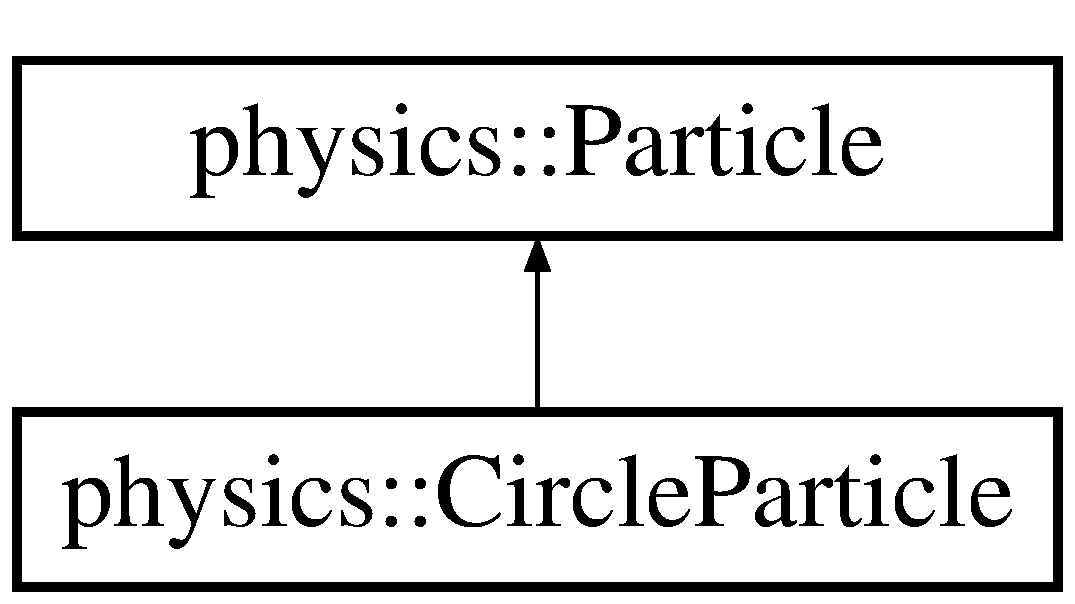
\includegraphics[height=2.000000cm]{classphysics_1_1_circle_particle}
\end{center}
\end{figure}
\subsection*{Métodos públicos}
\begin{DoxyCompactItemize}
\item 
\mbox{\hyperlink{classphysics_1_1_circle_particle_a3cf852542c435e3b051278b2c0a95e89}{Circle\+Particle}} ()
\begin{DoxyCompactList}\small\item\em Constructor por defecto de \mbox{\hyperlink{classphysics_1_1_particle_system}{Particle\+System}}. \end{DoxyCompactList}\item 
virtual void \mbox{\hyperlink{classphysics_1_1_circle_particle_a2d2c6b5715e99a4aca870327f0e38068}{Render}} (sf\+::\+Render\+Window \&window, bool active) override
\begin{DoxyCompactList}\small\item\em Renderiza la pat�cula con forma circular. \end{DoxyCompactList}\item 
virtual void \mbox{\hyperlink{classphysics_1_1_circle_particle_a6ac63df5e551d509793d6d09a1a0cd93}{Update}} (float delta\+\_\+time) override
\begin{DoxyCompactList}\small\item\em Atualiza la part�cula con forma circular. \end{DoxyCompactList}\end{DoxyCompactItemize}
\subsection*{Otros miembros heredados}


\subsection{Documentación del constructor y destructor}
\mbox{\Hypertarget{classphysics_1_1_circle_particle_a3cf852542c435e3b051278b2c0a95e89}\label{classphysics_1_1_circle_particle_a3cf852542c435e3b051278b2c0a95e89}} 
\index{physics\+::\+Circle\+Particle@{physics\+::\+Circle\+Particle}!Circle\+Particle@{Circle\+Particle}}
\index{Circle\+Particle@{Circle\+Particle}!physics\+::\+Circle\+Particle@{physics\+::\+Circle\+Particle}}
\subsubsection{\texorpdfstring{Circle\+Particle()}{CircleParticle()}}
{\footnotesize\ttfamily Circle\+Particle\+::\+Circle\+Particle (\begin{DoxyParamCaption}{ }\end{DoxyParamCaption})}



Constructor por defecto de \mbox{\hyperlink{classphysics_1_1_particle_system}{Particle\+System}}. 



\subsection{Documentación de las funciones miembro}
\mbox{\Hypertarget{classphysics_1_1_circle_particle_a2d2c6b5715e99a4aca870327f0e38068}\label{classphysics_1_1_circle_particle_a2d2c6b5715e99a4aca870327f0e38068}} 
\index{physics\+::\+Circle\+Particle@{physics\+::\+Circle\+Particle}!Render@{Render}}
\index{Render@{Render}!physics\+::\+Circle\+Particle@{physics\+::\+Circle\+Particle}}
\subsubsection{\texorpdfstring{Render()}{Render()}}
{\footnotesize\ttfamily void Circle\+Particle\+::\+Render (\begin{DoxyParamCaption}\item[{sf\+::\+Render\+Window \&}]{window,  }\item[{bool}]{active }\end{DoxyParamCaption})\hspace{0.3cm}{\ttfamily [override]}, {\ttfamily [virtual]}}



Renderiza la pat�cula con forma circular. 


\begin{DoxyParams}{Parámetros}
{\em window} & -\/$>$ es la ventana en donde se tiene que renderizar la pat�cula con forma circular \\
\hline
{\em active} & -\/$>$ Si es \char`\"{}true\char`\"{} significa que la part�cula con forma circular se debe renderizar \\
\hline
\end{DoxyParams}


Implementa \mbox{\hyperlink{classphysics_1_1_particle_a8e78d88c6e38d9a9cc9d5cc4a587358c}{physics\+::\+Particle}}.

\mbox{\Hypertarget{classphysics_1_1_circle_particle_a6ac63df5e551d509793d6d09a1a0cd93}\label{classphysics_1_1_circle_particle_a6ac63df5e551d509793d6d09a1a0cd93}} 
\index{physics\+::\+Circle\+Particle@{physics\+::\+Circle\+Particle}!Update@{Update}}
\index{Update@{Update}!physics\+::\+Circle\+Particle@{physics\+::\+Circle\+Particle}}
\subsubsection{\texorpdfstring{Update()}{Update()}}
{\footnotesize\ttfamily void Circle\+Particle\+::\+Update (\begin{DoxyParamCaption}\item[{float}]{delta\+\_\+time }\end{DoxyParamCaption})\hspace{0.3cm}{\ttfamily [override]}, {\ttfamily [virtual]}}



Atualiza la part�cula con forma circular. 


\begin{DoxyParams}{Parámetros}
{\em delta\+\_\+time} & -\/$>$ son los segundos por frame \\
\hline
\end{DoxyParams}


Implementa \mbox{\hyperlink{classphysics_1_1_particle_ac44f133ed437b12914828315efeea79f}{physics\+::\+Particle}}.



La documentación para esta clase fue generada a partir de los siguientes ficheros\+:\begin{DoxyCompactItemize}
\item 
\mbox{\hyperlink{_circle_particle_8hpp}{Circle\+Particle.\+hpp}}\item 
\mbox{\hyperlink{_circle_particle_8cpp}{Circle\+Particle.\+cpp}}\end{DoxyCompactItemize}

\hypertarget{class_circle_particle}{}\section{Referencia de la Clase Circle\+Particle}
\label{class_circle_particle}\index{Circle\+Particle@{Circle\+Particle}}


Clase en donde se renderizan y updatean las part�cular con forma redondeada, hereda de la clase \char`\"{}\+Particle\char`\"{}.  




{\ttfamily \#include $<$Circle\+Particle.\+hpp$>$}



\subsection{Descripción detallada}
Clase en donde se renderizan y updatean las part�cular con forma redondeada, hereda de la clase \char`\"{}\+Particle\char`\"{}. 

La documentación para esta clase fue generada a partir del siguiente fichero\+:\begin{DoxyCompactItemize}
\item 
\mbox{\hyperlink{_circle_particle_8hpp}{Circle\+Particle.\+hpp}}\end{DoxyCompactItemize}

\hypertarget{class_collision}{}\section{Referencia de la Clase Collision}
\label{class_collision}\index{Collision@{Collision}}


Clase en donde se llaman a las colisiones de los objetos con otros.  




{\ttfamily \#include $<$Collision.\+hpp$>$}



\subsection{Descripción detallada}
Clase en donde se llaman a las colisiones de los objetos con otros. 

La documentación para esta clase fue generada a partir del siguiente fichero\+:\begin{DoxyCompactItemize}
\item 
\mbox{\hyperlink{_collision_8hpp}{Collision.\+hpp}}\end{DoxyCompactItemize}

\hypertarget{classphysics_1_1_collison}{}\section{Referencia de la Clase physics\+:\+:Collison}
\label{classphysics_1_1_collison}\index{physics\+::\+Collison@{physics\+::\+Collison}}


{\ttfamily \#include $<$Collision.\+hpp$>$}

Diagrama de herencias de physics\+:\+:Collison\begin{figure}[H]
\begin{center}
\leavevmode
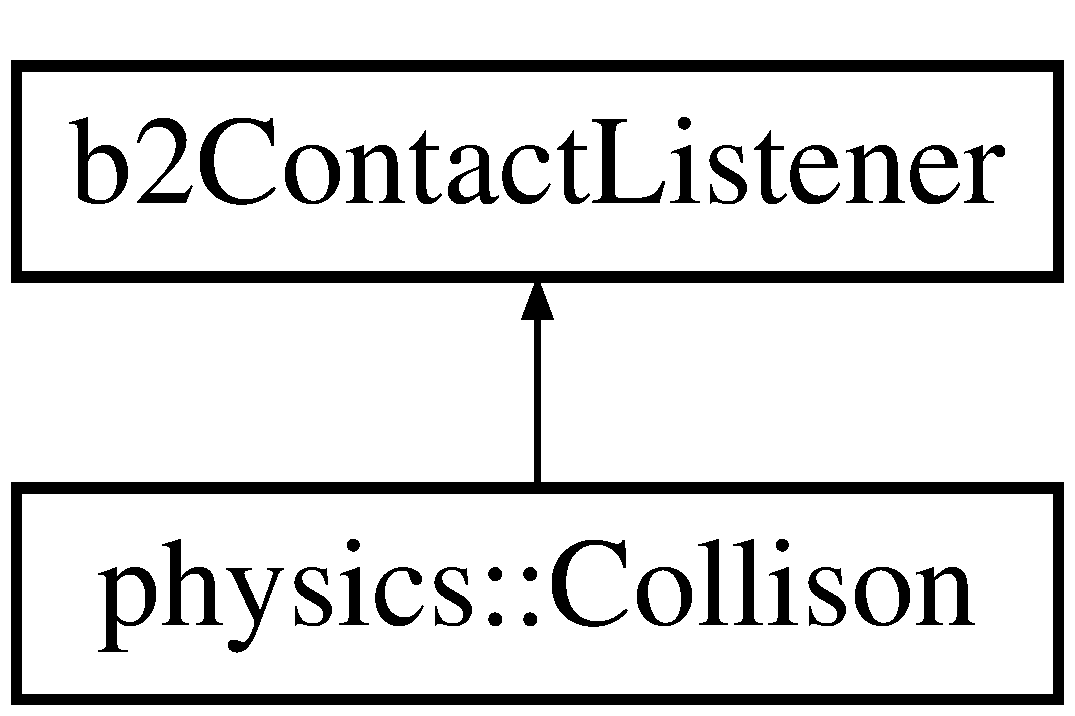
\includegraphics[height=2.000000cm]{classphysics_1_1_collison}
\end{center}
\end{figure}
\subsection*{Métodos públicos}
\begin{DoxyCompactItemize}
\item 
void \mbox{\hyperlink{classphysics_1_1_collison_aa24b202d58a20f9c088d06f62e699b67}{Begin\+Contact}} (b2\+Contact $\ast$contact)
\begin{DoxyCompactList}\small\item\em Se ejecuta cuando un objeto empieza a colisionar con otro. \end{DoxyCompactList}\item 
void \mbox{\hyperlink{classphysics_1_1_collison_a0c31a5688fbb7ecfbf866e52a1c5e817}{End\+Contact}} (b2\+Contact $\ast$contact)
\begin{DoxyCompactList}\small\item\em Se ejecuta cuando un objeto termina de colisionar con otro. \end{DoxyCompactList}\end{DoxyCompactItemize}


\subsection{Documentación de las funciones miembro}
\mbox{\Hypertarget{classphysics_1_1_collison_aa24b202d58a20f9c088d06f62e699b67}\label{classphysics_1_1_collison_aa24b202d58a20f9c088d06f62e699b67}} 
\index{physics\+::\+Collison@{physics\+::\+Collison}!Begin\+Contact@{Begin\+Contact}}
\index{Begin\+Contact@{Begin\+Contact}!physics\+::\+Collison@{physics\+::\+Collison}}
\subsubsection{\texorpdfstring{Begin\+Contact()}{BeginContact()}}
{\footnotesize\ttfamily void physics\+::\+Collison\+::\+Begin\+Contact (\begin{DoxyParamCaption}\item[{b2\+Contact $\ast$}]{contact }\end{DoxyParamCaption})\hspace{0.3cm}{\ttfamily [inline]}}



Se ejecuta cuando un objeto empieza a colisionar con otro. 


\begin{DoxyParams}{Parámetros}
{\em contact} & -\/$>$ contiene toda la informaci�n de la colisi�n entre los objetos \\
\hline
\end{DoxyParams}
\mbox{\Hypertarget{classphysics_1_1_collison_a0c31a5688fbb7ecfbf866e52a1c5e817}\label{classphysics_1_1_collison_a0c31a5688fbb7ecfbf866e52a1c5e817}} 
\index{physics\+::\+Collison@{physics\+::\+Collison}!End\+Contact@{End\+Contact}}
\index{End\+Contact@{End\+Contact}!physics\+::\+Collison@{physics\+::\+Collison}}
\subsubsection{\texorpdfstring{End\+Contact()}{EndContact()}}
{\footnotesize\ttfamily void physics\+::\+Collison\+::\+End\+Contact (\begin{DoxyParamCaption}\item[{b2\+Contact $\ast$}]{contact }\end{DoxyParamCaption})\hspace{0.3cm}{\ttfamily [inline]}}



Se ejecuta cuando un objeto termina de colisionar con otro. 


\begin{DoxyParams}{Parámetros}
{\em contact} & -\/$>$ contiene toda la informaci�n de la colisi�n entre los objetos \\
\hline
\end{DoxyParams}


La documentación para esta clase fue generada a partir del siguiente fichero\+:\begin{DoxyCompactItemize}
\item 
\mbox{\hyperlink{_collision_8hpp}{Collision.\+hpp}}\end{DoxyCompactItemize}

\hypertarget{classphysics_1_1_particle}{}\section{Referencia de la Clase physics\+:\+:Particle}
\label{classphysics_1_1_particle}\index{physics\+::\+Particle@{physics\+::\+Particle}}


{\ttfamily \#include $<$Particle.\+hpp$>$}

Diagrama de herencias de physics\+:\+:Particle\begin{figure}[H]
\begin{center}
\leavevmode
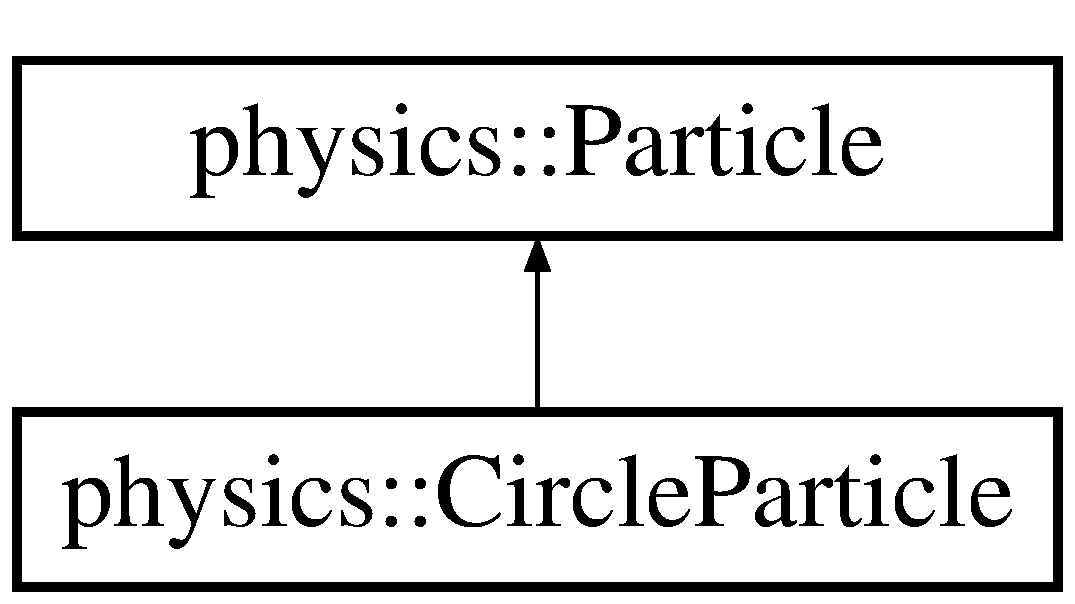
\includegraphics[height=2.000000cm]{classphysics_1_1_particle}
\end{center}
\end{figure}
\subsection*{Métodos públicos}
\begin{DoxyCompactItemize}
\item 
virtual void \mbox{\hyperlink{classphysics_1_1_particle_a8e78d88c6e38d9a9cc9d5cc4a587358c}{Render}} (sf\+::\+Render\+Window \&window, bool active)=0
\begin{DoxyCompactList}\small\item\em Renderiza la part�cula, es un m�todo virtual. \end{DoxyCompactList}\item 
virtual void \mbox{\hyperlink{classphysics_1_1_particle_ac44f133ed437b12914828315efeea79f}{Update}} (float delta\+\_\+time)=0
\begin{DoxyCompactList}\small\item\em Atualiza la part�cula, es un m�todo virtual. \end{DoxyCompactList}\end{DoxyCompactItemize}
\subsection*{Atributos públicos}
\begin{DoxyCompactItemize}
\item 
float \mbox{\hyperlink{classphysics_1_1_particle_ad017940d860da63b3711128ef86c1f21}{start\+Time}} = 0
\begin{DoxyCompactList}\small\item\em Act�a de timer, y su valor inicial es 0. \end{DoxyCompactList}\item 
float \mbox{\hyperlink{classphysics_1_1_particle_aca4d2b2baf199876559b7dac338e68ba}{life\+Time}}
\begin{DoxyCompactList}\small\item\em El tiempo de vida de la part�cula. \end{DoxyCompactList}\item 
sf\+::\+Vector2f \mbox{\hyperlink{classphysics_1_1_particle_a3d04ce30ecddcca0a2c70b75383ec8d8}{start\+Position}}
\begin{DoxyCompactList}\small\item\em La posici�n inicial de la part�cula. \end{DoxyCompactList}\item 
sf\+::\+Vector2f \mbox{\hyperlink{classphysics_1_1_particle_a1d0a0aca61f011c98d68675ff5a16782}{position}}
\begin{DoxyCompactList}\small\item\em La posici�n actual de la part�cula. \end{DoxyCompactList}\item 
sf\+::\+Vector2f \mbox{\hyperlink{classphysics_1_1_particle_a4f5fc3f2be3f829ba2108aa4c46d8686}{velocity}}
\begin{DoxyCompactList}\small\item\em La velocidad inicial y actual de la part�cula. \end{DoxyCompactList}\item 
sf\+::\+Shape $\ast$ \mbox{\hyperlink{classphysics_1_1_particle_a18923a7446d8242155a8dc0728db4a00}{shape}}
\begin{DoxyCompactList}\small\item\em Puntero a la forma gr�fica de la part�cula. \end{DoxyCompactList}\end{DoxyCompactItemize}


\subsection{Documentación de las funciones miembro}
\mbox{\Hypertarget{classphysics_1_1_particle_a8e78d88c6e38d9a9cc9d5cc4a587358c}\label{classphysics_1_1_particle_a8e78d88c6e38d9a9cc9d5cc4a587358c}} 
\index{physics\+::\+Particle@{physics\+::\+Particle}!Render@{Render}}
\index{Render@{Render}!physics\+::\+Particle@{physics\+::\+Particle}}
\subsubsection{\texorpdfstring{Render()}{Render()}}
{\footnotesize\ttfamily virtual void physics\+::\+Particle\+::\+Render (\begin{DoxyParamCaption}\item[{sf\+::\+Render\+Window \&}]{window,  }\item[{bool}]{active }\end{DoxyParamCaption})\hspace{0.3cm}{\ttfamily [pure virtual]}}



Renderiza la part�cula, es un m�todo virtual. 


\begin{DoxyParams}{Parámetros}
{\em window} & -\/$>$ es la ventana en donde se tiene que renderizar la pat�cula \\
\hline
{\em active} & -\/$>$ Si es \char`\"{}true\char`\"{} significa que la part�cula se debe renderizar \\
\hline
\end{DoxyParams}


Implementado en \mbox{\hyperlink{classphysics_1_1_circle_particle_a2d2c6b5715e99a4aca870327f0e38068}{physics\+::\+Circle\+Particle}}.

\mbox{\Hypertarget{classphysics_1_1_particle_ac44f133ed437b12914828315efeea79f}\label{classphysics_1_1_particle_ac44f133ed437b12914828315efeea79f}} 
\index{physics\+::\+Particle@{physics\+::\+Particle}!Update@{Update}}
\index{Update@{Update}!physics\+::\+Particle@{physics\+::\+Particle}}
\subsubsection{\texorpdfstring{Update()}{Update()}}
{\footnotesize\ttfamily virtual void physics\+::\+Particle\+::\+Update (\begin{DoxyParamCaption}\item[{float}]{delta\+\_\+time }\end{DoxyParamCaption})\hspace{0.3cm}{\ttfamily [pure virtual]}}



Atualiza la part�cula, es un m�todo virtual. 


\begin{DoxyParams}{Parámetros}
{\em delta\+\_\+time} & -\/$>$ son los segundos por frame \\
\hline
\end{DoxyParams}


Implementado en \mbox{\hyperlink{classphysics_1_1_circle_particle_a6ac63df5e551d509793d6d09a1a0cd93}{physics\+::\+Circle\+Particle}}.



\subsection{Documentación de los datos miembro}
\mbox{\Hypertarget{classphysics_1_1_particle_aca4d2b2baf199876559b7dac338e68ba}\label{classphysics_1_1_particle_aca4d2b2baf199876559b7dac338e68ba}} 
\index{physics\+::\+Particle@{physics\+::\+Particle}!life\+Time@{life\+Time}}
\index{life\+Time@{life\+Time}!physics\+::\+Particle@{physics\+::\+Particle}}
\subsubsection{\texorpdfstring{life\+Time}{lifeTime}}
{\footnotesize\ttfamily float physics\+::\+Particle\+::life\+Time}



El tiempo de vida de la part�cula. 

\mbox{\Hypertarget{classphysics_1_1_particle_a1d0a0aca61f011c98d68675ff5a16782}\label{classphysics_1_1_particle_a1d0a0aca61f011c98d68675ff5a16782}} 
\index{physics\+::\+Particle@{physics\+::\+Particle}!position@{position}}
\index{position@{position}!physics\+::\+Particle@{physics\+::\+Particle}}
\subsubsection{\texorpdfstring{position}{position}}
{\footnotesize\ttfamily sf\+::\+Vector2f physics\+::\+Particle\+::position}



La posici�n actual de la part�cula. 

\mbox{\Hypertarget{classphysics_1_1_particle_a18923a7446d8242155a8dc0728db4a00}\label{classphysics_1_1_particle_a18923a7446d8242155a8dc0728db4a00}} 
\index{physics\+::\+Particle@{physics\+::\+Particle}!shape@{shape}}
\index{shape@{shape}!physics\+::\+Particle@{physics\+::\+Particle}}
\subsubsection{\texorpdfstring{shape}{shape}}
{\footnotesize\ttfamily sf\+::\+Shape$\ast$ physics\+::\+Particle\+::shape}



Puntero a la forma gr�fica de la part�cula. 

\mbox{\Hypertarget{classphysics_1_1_particle_a3d04ce30ecddcca0a2c70b75383ec8d8}\label{classphysics_1_1_particle_a3d04ce30ecddcca0a2c70b75383ec8d8}} 
\index{physics\+::\+Particle@{physics\+::\+Particle}!start\+Position@{start\+Position}}
\index{start\+Position@{start\+Position}!physics\+::\+Particle@{physics\+::\+Particle}}
\subsubsection{\texorpdfstring{start\+Position}{startPosition}}
{\footnotesize\ttfamily sf\+::\+Vector2f physics\+::\+Particle\+::start\+Position}



La posici�n inicial de la part�cula. 

\mbox{\Hypertarget{classphysics_1_1_particle_ad017940d860da63b3711128ef86c1f21}\label{classphysics_1_1_particle_ad017940d860da63b3711128ef86c1f21}} 
\index{physics\+::\+Particle@{physics\+::\+Particle}!start\+Time@{start\+Time}}
\index{start\+Time@{start\+Time}!physics\+::\+Particle@{physics\+::\+Particle}}
\subsubsection{\texorpdfstring{start\+Time}{startTime}}
{\footnotesize\ttfamily float physics\+::\+Particle\+::start\+Time = 0}



Act�a de timer, y su valor inicial es 0. 

\mbox{\Hypertarget{classphysics_1_1_particle_a4f5fc3f2be3f829ba2108aa4c46d8686}\label{classphysics_1_1_particle_a4f5fc3f2be3f829ba2108aa4c46d8686}} 
\index{physics\+::\+Particle@{physics\+::\+Particle}!velocity@{velocity}}
\index{velocity@{velocity}!physics\+::\+Particle@{physics\+::\+Particle}}
\subsubsection{\texorpdfstring{velocity}{velocity}}
{\footnotesize\ttfamily sf\+::\+Vector2f physics\+::\+Particle\+::velocity}



La velocidad inicial y actual de la part�cula. 



La documentación para esta clase fue generada a partir del siguiente fichero\+:\begin{DoxyCompactItemize}
\item 
\mbox{\hyperlink{_particle_8hpp}{Particle.\+hpp}}\end{DoxyCompactItemize}

\hypertarget{class_particle}{}\section{Referencia de la Clase Particle}
\label{class_particle}\index{Particle@{Particle}}


Clase abstracta en donde se definen m�todos y variables de una part�cula.  




{\ttfamily \#include $<$Particle.\+hpp$>$}



\subsection{Descripción detallada}
Clase abstracta en donde se definen m�todos y variables de una part�cula. 

La documentación para esta clase fue generada a partir del siguiente fichero\+:\begin{DoxyCompactItemize}
\item 
\mbox{\hyperlink{_particle_8hpp}{Particle.\+hpp}}\end{DoxyCompactItemize}

\hypertarget{classphysics_1_1_particle_system}{}\section{Referencia de la plantilla de la Clase physics\+:\+:Particle\+System$<$ P\+A\+R\+T\+I\+C\+LE $>$}
\label{classphysics_1_1_particle_system}\index{physics\+::\+Particle\+System$<$ P\+A\+R\+T\+I\+C\+L\+E $>$@{physics\+::\+Particle\+System$<$ P\+A\+R\+T\+I\+C\+L\+E $>$}}


{\ttfamily \#include $<$Particle\+System.\+hpp$>$}

\subsection*{Métodos públicos}
\begin{DoxyCompactItemize}
\item 
\mbox{\hyperlink{classphysics_1_1_particle_system_a8739be0be3c82af68f324521703735d8}{Particle\+System}} ()
\begin{DoxyCompactList}\small\item\em Constructor por defecto de \mbox{\hyperlink{classphysics_1_1_particle_system}{Particle\+System}}. \end{DoxyCompactList}\item 
\mbox{\hyperlink{classphysics_1_1_particle_system_a584f1c968c76588c17de0da2e511f6e8}{Particle\+System}} (int particle\+Count, sf\+::\+Vector2f life\+Time, sf\+::\+Vector2f Particle\+System\+Position, sf\+::\+Vector2f x\+Position\+Offset, sf\+::\+Vector2f y\+Position\+Offset, sf\+::\+Vector2f Particle\+System\+Velocity, sf\+::\+Vector2f x\+Velocity\+Offset, sf\+::\+Vector2f y\+Velocity\+Offset)
\begin{DoxyCompactList}\small\item\em Renderiza la escena. \end{DoxyCompactList}\item 
void \mbox{\hyperlink{classphysics_1_1_particle_system_aed8455c353e3ee0fcc4e1bb167c91d95}{Render}} (sf\+::\+Render\+Window \&window, bool Particle\+System\+Active)
\begin{DoxyCompactList}\small\item\em Renderiza el sistema de part�culas. \end{DoxyCompactList}\item 
void \mbox{\hyperlink{classphysics_1_1_particle_system_ae217afe8b9b47d8a7a8b0055326606c4}{Update}} (float delta\+\_\+time)
\begin{DoxyCompactList}\small\item\em Atualiza el sistema de part�culas. \end{DoxyCompactList}\item 
float \mbox{\hyperlink{classphysics_1_1_particle_system_aac097412188bb8be886f86329109dd7b}{get\+Ramdom\+Float}} (float a, float b)
\begin{DoxyCompactList}\small\item\em Calcula un n�mero aleatorio entre el rango de los par�metros y lo devuelve. \end{DoxyCompactList}\end{DoxyCompactItemize}
\subsection*{Atributos públicos}
\begin{DoxyCompactItemize}
\item 
std\+::vector$<$ P\+A\+R\+T\+I\+C\+LE $>$ \mbox{\hyperlink{classphysics_1_1_particle_system_a9bd70b33a15bc7141aba39b23d737005}{particles}}
\begin{DoxyCompactList}\small\item\em Un vector de todas las pert�culas que pertenecen al mismo sistema de part�culas. \end{DoxyCompactList}\end{DoxyCompactItemize}


\subsection{Documentación del constructor y destructor}
\mbox{\Hypertarget{classphysics_1_1_particle_system_a8739be0be3c82af68f324521703735d8}\label{classphysics_1_1_particle_system_a8739be0be3c82af68f324521703735d8}} 
\index{physics\+::\+Particle\+System@{physics\+::\+Particle\+System}!Particle\+System@{Particle\+System}}
\index{Particle\+System@{Particle\+System}!physics\+::\+Particle\+System@{physics\+::\+Particle\+System}}
\subsubsection{\texorpdfstring{Particle\+System()}{ParticleSystem()}\hspace{0.1cm}{\footnotesize\ttfamily [1/2]}}
{\footnotesize\ttfamily template$<$typename P\+A\+R\+T\+I\+C\+LE$>$ \\
\mbox{\hyperlink{classphysics_1_1_particle_system}{physics\+::\+Particle\+System}}$<$ P\+A\+R\+T\+I\+C\+LE $>$\+::\mbox{\hyperlink{classphysics_1_1_particle_system}{Particle\+System}} (\begin{DoxyParamCaption}{ }\end{DoxyParamCaption})\hspace{0.3cm}{\ttfamily [inline]}}



Constructor por defecto de \mbox{\hyperlink{classphysics_1_1_particle_system}{Particle\+System}}. 

\mbox{\Hypertarget{classphysics_1_1_particle_system_a584f1c968c76588c17de0da2e511f6e8}\label{classphysics_1_1_particle_system_a584f1c968c76588c17de0da2e511f6e8}} 
\index{physics\+::\+Particle\+System@{physics\+::\+Particle\+System}!Particle\+System@{Particle\+System}}
\index{Particle\+System@{Particle\+System}!physics\+::\+Particle\+System@{physics\+::\+Particle\+System}}
\subsubsection{\texorpdfstring{Particle\+System()}{ParticleSystem()}\hspace{0.1cm}{\footnotesize\ttfamily [2/2]}}
{\footnotesize\ttfamily template$<$typename P\+A\+R\+T\+I\+C\+LE$>$ \\
\mbox{\hyperlink{classphysics_1_1_particle_system}{physics\+::\+Particle\+System}}$<$ P\+A\+R\+T\+I\+C\+LE $>$\+::\mbox{\hyperlink{classphysics_1_1_particle_system}{Particle\+System}} (\begin{DoxyParamCaption}\item[{int}]{particle\+Count,  }\item[{sf\+::\+Vector2f}]{life\+Time,  }\item[{sf\+::\+Vector2f}]{Particle\+System\+Position,  }\item[{sf\+::\+Vector2f}]{x\+Position\+Offset,  }\item[{sf\+::\+Vector2f}]{y\+Position\+Offset,  }\item[{sf\+::\+Vector2f}]{Particle\+System\+Velocity,  }\item[{sf\+::\+Vector2f}]{x\+Velocity\+Offset,  }\item[{sf\+::\+Vector2f}]{y\+Velocity\+Offset }\end{DoxyParamCaption})\hspace{0.3cm}{\ttfamily [inline]}}



Renderiza la escena. 


\begin{DoxyParams}{Parámetros}
{\em particle\+Count} & -\/$>$ el n�mero de part�culas que va a tener el sistema de part�culas \\
\hline
{\em life\+Time} & -\/$>$ el tiempo de vida del sistema de part�culas \\
\hline
{\em Particle\+System\+Position} & -\/$>$ la posici�n del sistema de part�culas \\
\hline
{\em x\+Position\+Offset} & -\/$>$ los offsets de la posici�n del eje X del sistema de part�culas \\
\hline
{\em y\+Position\+Offset} & -\/$>$ los offsets de la posici�n del eje Y del sistema de part�culas \\
\hline
{\em Particle\+System\+Velocity} & -\/$>$ la velocidad del sistema de part�culas \\
\hline
{\em x\+Velocity\+Offset} & -\/$>$ los offsets de la velocidad del eje X del sistema de part�culas \\
\hline
{\em y\+Velocity\+Offset} & -\/$>$ los offsets de la velocidad del eje Y del sistema de part�culas \\
\hline
\end{DoxyParams}


\subsection{Documentación de las funciones miembro}
\mbox{\Hypertarget{classphysics_1_1_particle_system_aac097412188bb8be886f86329109dd7b}\label{classphysics_1_1_particle_system_aac097412188bb8be886f86329109dd7b}} 
\index{physics\+::\+Particle\+System@{physics\+::\+Particle\+System}!get\+Ramdom\+Float@{get\+Ramdom\+Float}}
\index{get\+Ramdom\+Float@{get\+Ramdom\+Float}!physics\+::\+Particle\+System@{physics\+::\+Particle\+System}}
\subsubsection{\texorpdfstring{get\+Ramdom\+Float()}{getRamdomFloat()}}
{\footnotesize\ttfamily template$<$typename P\+A\+R\+T\+I\+C\+LE$>$ \\
float \mbox{\hyperlink{classphysics_1_1_particle_system}{physics\+::\+Particle\+System}}$<$ P\+A\+R\+T\+I\+C\+LE $>$\+::get\+Ramdom\+Float (\begin{DoxyParamCaption}\item[{float}]{a,  }\item[{float}]{b }\end{DoxyParamCaption})\hspace{0.3cm}{\ttfamily [inline]}}



Calcula un n�mero aleatorio entre el rango de los par�metros y lo devuelve. 


\begin{DoxyParams}{Parámetros}
{\em a} & -\/$>$ el n�mero m�nimo del rango \\
\hline
{\em b} & -\/$>$ el n�mero m�ximo del rango \\
\hline
\end{DoxyParams}
\mbox{\Hypertarget{classphysics_1_1_particle_system_aed8455c353e3ee0fcc4e1bb167c91d95}\label{classphysics_1_1_particle_system_aed8455c353e3ee0fcc4e1bb167c91d95}} 
\index{physics\+::\+Particle\+System@{physics\+::\+Particle\+System}!Render@{Render}}
\index{Render@{Render}!physics\+::\+Particle\+System@{physics\+::\+Particle\+System}}
\subsubsection{\texorpdfstring{Render()}{Render()}}
{\footnotesize\ttfamily template$<$typename P\+A\+R\+T\+I\+C\+LE$>$ \\
void \mbox{\hyperlink{classphysics_1_1_particle_system}{physics\+::\+Particle\+System}}$<$ P\+A\+R\+T\+I\+C\+LE $>$\+::Render (\begin{DoxyParamCaption}\item[{sf\+::\+Render\+Window \&}]{window,  }\item[{bool}]{Particle\+System\+Active }\end{DoxyParamCaption})\hspace{0.3cm}{\ttfamily [inline]}}



Renderiza el sistema de part�culas. 


\begin{DoxyParams}{Parámetros}
{\em window} & -\/$>$ es la ventana en donde se tiene que renderizar la escena \\
\hline
{\em Particle\+System\+Active} & -\/$>$ Si es \char`\"{}true\char`\"{} significa que el sistema de part�culas se debe renderizar \\
\hline
\end{DoxyParams}
\mbox{\Hypertarget{classphysics_1_1_particle_system_ae217afe8b9b47d8a7a8b0055326606c4}\label{classphysics_1_1_particle_system_ae217afe8b9b47d8a7a8b0055326606c4}} 
\index{physics\+::\+Particle\+System@{physics\+::\+Particle\+System}!Update@{Update}}
\index{Update@{Update}!physics\+::\+Particle\+System@{physics\+::\+Particle\+System}}
\subsubsection{\texorpdfstring{Update()}{Update()}}
{\footnotesize\ttfamily template$<$typename P\+A\+R\+T\+I\+C\+LE$>$ \\
void \mbox{\hyperlink{classphysics_1_1_particle_system}{physics\+::\+Particle\+System}}$<$ P\+A\+R\+T\+I\+C\+LE $>$\+::Update (\begin{DoxyParamCaption}\item[{float}]{delta\+\_\+time }\end{DoxyParamCaption})\hspace{0.3cm}{\ttfamily [inline]}}



Atualiza el sistema de part�culas. 


\begin{DoxyParams}{Parámetros}
{\em delta\+\_\+time} & -\/$>$ son los segundos por frame \\
\hline
\end{DoxyParams}


\subsection{Documentación de los datos miembro}
\mbox{\Hypertarget{classphysics_1_1_particle_system_a9bd70b33a15bc7141aba39b23d737005}\label{classphysics_1_1_particle_system_a9bd70b33a15bc7141aba39b23d737005}} 
\index{physics\+::\+Particle\+System@{physics\+::\+Particle\+System}!particles@{particles}}
\index{particles@{particles}!physics\+::\+Particle\+System@{physics\+::\+Particle\+System}}
\subsubsection{\texorpdfstring{particles}{particles}}
{\footnotesize\ttfamily template$<$typename P\+A\+R\+T\+I\+C\+LE$>$ \\
std\+::vector$<$P\+A\+R\+T\+I\+C\+LE$>$ \mbox{\hyperlink{classphysics_1_1_particle_system}{physics\+::\+Particle\+System}}$<$ P\+A\+R\+T\+I\+C\+LE $>$\+::particles}



Un vector de todas las pert�culas que pertenecen al mismo sistema de part�culas. 



La documentación para esta clase fue generada a partir del siguiente fichero\+:\begin{DoxyCompactItemize}
\item 
\mbox{\hyperlink{_particle_system_8hpp}{Particle\+System.\+hpp}}\end{DoxyCompactItemize}

\hypertarget{class_particle_system}{}\section{Referencia de la Clase Particle\+System}
\label{class_particle_system}\index{Particle\+System@{Particle\+System}}


Clase que se encarga de montar el sistema de part�culas, renderizarlo y updatearlo.  




{\ttfamily \#include $<$Particle\+System.\+hpp$>$}



\subsection{Descripción detallada}
Clase que se encarga de montar el sistema de part�culas, renderizarlo y updatearlo. 

La documentación para esta clase fue generada a partir del siguiente fichero\+:\begin{DoxyCompactItemize}
\item 
\mbox{\hyperlink{_particle_system_8hpp}{Particle\+System.\+hpp}}\end{DoxyCompactItemize}

\hypertarget{classphysics_1_1_scene}{}\section{Referencia de la Clase physics\+:\+:Scene}
\label{classphysics_1_1_scene}\index{physics\+::\+Scene@{physics\+::\+Scene}}


{\ttfamily \#include $<$Scene.\+hpp$>$}

\subsection*{Métodos públicos}
\begin{DoxyCompactItemize}
\item 
\mbox{\hyperlink{classphysics_1_1_scene_ac034b284d50291c66ef8553001e37fb2}{Scene}} (b2\+Vec2 gravity=b2\+Vec2\{ 0, -\/9.\+8f \})
\begin{DoxyCompactList}\small\item\em Constructor de la escena. \end{DoxyCompactList}\item 
\mbox{\hyperlink{classphysics_1_1_scene_a3b8cec2e32546713915f8c6303c951f1}{$\sim$\+Scene}} ()
\begin{DoxyCompactList}\small\item\em Desontructor de la escena. \end{DoxyCompactList}\item 
void \mbox{\hyperlink{classphysics_1_1_scene_afc5239f30d0ee1d542bc1f4e3a8cbf63}{Update}} (float delta\+\_\+time)
\begin{DoxyCompactList}\small\item\em Atualiza la escena. \end{DoxyCompactList}\item 
void \mbox{\hyperlink{classphysics_1_1_scene_ab86f3c5e0389b5ef13a5b5047fcc1b94}{Render}} (sf\+::\+Render\+Window \&window)
\begin{DoxyCompactList}\small\item\em Renderiza la escena. \end{DoxyCompactList}\end{DoxyCompactItemize}
\subsection*{Atributos públicos}
\begin{DoxyCompactItemize}
\item 
std\+::map$<$ std\+::string, std\+::shared\+\_\+ptr$<$ \mbox{\hyperlink{classphysics_1_1_box2_d_object}{Box2\+D\+Object}} $>$ $>$ \mbox{\hyperlink{classphysics_1_1_scene_a9e3e902466f5d6d4aa81c1db3920af4e}{scene\+Objects}}
\begin{DoxyCompactList}\small\item\em Contine todos los \char`\"{}\+Box2\+D\+Object\char`\"{} de la escena. \end{DoxyCompactList}\item 
b2\+World $\ast$ \mbox{\hyperlink{classphysics_1_1_scene_a33797c64e136e212027672fade6cc30a}{box2\+D\+World}}
\begin{DoxyCompactList}\small\item\em Un puntero al mundo. \end{DoxyCompactList}\item 
\mbox{\hyperlink{namespacephysics_a962adae29e6ee31067fabcf90eb01dac}{Circle\+Particle\+System}} \mbox{\hyperlink{classphysics_1_1_scene_a21559bc49a1dbeb0fede231f35072b66}{particle\+System}}
\begin{DoxyCompactList}\small\item\em Sistema del part�culas de part�culas redondas. \end{DoxyCompactList}\item 
std\+::shared\+\_\+ptr$<$ \mbox{\hyperlink{classphysics_1_1_box2_d_object}{Box2\+D\+Object}} $>$ \mbox{\hyperlink{classphysics_1_1_scene_af7834c449556f5ca56703abd81ca8ddc}{ball}}
\begin{DoxyCompactList}\small\item\em Puntero al \char`\"{}\+Box2\+D\+Object\char`\"{} de la escena cuyo tag es \char`\"{}ball\char`\"{}. \end{DoxyCompactList}\item 
bool \mbox{\hyperlink{classphysics_1_1_scene_add6ec396d473e5dae5bf068e720dd8c6}{particle\+System\+Active}}
\begin{DoxyCompactList}\small\item\em Si es \char`\"{}true\char`\"{} significa que la \char`\"{}ball\char`\"{} se debe resetear. \end{DoxyCompactList}\end{DoxyCompactItemize}


\subsection{Documentación del constructor y destructor}
\mbox{\Hypertarget{classphysics_1_1_scene_ac034b284d50291c66ef8553001e37fb2}\label{classphysics_1_1_scene_ac034b284d50291c66ef8553001e37fb2}} 
\index{physics\+::\+Scene@{physics\+::\+Scene}!Scene@{Scene}}
\index{Scene@{Scene}!physics\+::\+Scene@{physics\+::\+Scene}}
\subsubsection{\texorpdfstring{Scene()}{Scene()}}
{\footnotesize\ttfamily Scene\+::\+Scene (\begin{DoxyParamCaption}\item[{b2\+Vec2}]{gravity = {\ttfamily b2Vec2\{~0,~-\/9.8f~\}} }\end{DoxyParamCaption})}



Constructor de la escena. 


\begin{DoxyParams}{Parámetros}
{\em gravity} & -\/$>$ gravedad del mundo, por defecto es de -\/9.\+8 en el eje Y \\
\hline
\end{DoxyParams}
\mbox{\Hypertarget{classphysics_1_1_scene_a3b8cec2e32546713915f8c6303c951f1}\label{classphysics_1_1_scene_a3b8cec2e32546713915f8c6303c951f1}} 
\index{physics\+::\+Scene@{physics\+::\+Scene}!````~Scene@{$\sim$\+Scene}}
\index{````~Scene@{$\sim$\+Scene}!physics\+::\+Scene@{physics\+::\+Scene}}
\subsubsection{\texorpdfstring{$\sim$\+Scene()}{~Scene()}}
{\footnotesize\ttfamily Scene\+::$\sim$\+Scene (\begin{DoxyParamCaption}{ }\end{DoxyParamCaption})}



Desontructor de la escena. 



\subsection{Documentación de las funciones miembro}
\mbox{\Hypertarget{classphysics_1_1_scene_ab86f3c5e0389b5ef13a5b5047fcc1b94}\label{classphysics_1_1_scene_ab86f3c5e0389b5ef13a5b5047fcc1b94}} 
\index{physics\+::\+Scene@{physics\+::\+Scene}!Render@{Render}}
\index{Render@{Render}!physics\+::\+Scene@{physics\+::\+Scene}}
\subsubsection{\texorpdfstring{Render()}{Render()}}
{\footnotesize\ttfamily void Scene\+::\+Render (\begin{DoxyParamCaption}\item[{sf\+::\+Render\+Window \&}]{window }\end{DoxyParamCaption})}



Renderiza la escena. 


\begin{DoxyParams}{Parámetros}
{\em window} & -\/$>$ es la ventana en donde se tiene que renderizar la escena \\
\hline
\end{DoxyParams}
\mbox{\Hypertarget{classphysics_1_1_scene_afc5239f30d0ee1d542bc1f4e3a8cbf63}\label{classphysics_1_1_scene_afc5239f30d0ee1d542bc1f4e3a8cbf63}} 
\index{physics\+::\+Scene@{physics\+::\+Scene}!Update@{Update}}
\index{Update@{Update}!physics\+::\+Scene@{physics\+::\+Scene}}
\subsubsection{\texorpdfstring{Update()}{Update()}}
{\footnotesize\ttfamily void Scene\+::\+Update (\begin{DoxyParamCaption}\item[{float}]{delta\+\_\+time }\end{DoxyParamCaption})}



Atualiza la escena. 


\begin{DoxyParams}{Parámetros}
{\em delta\+\_\+time} & -\/$>$ son los segundos por frame \\
\hline
\end{DoxyParams}


\subsection{Documentación de los datos miembro}
\mbox{\Hypertarget{classphysics_1_1_scene_af7834c449556f5ca56703abd81ca8ddc}\label{classphysics_1_1_scene_af7834c449556f5ca56703abd81ca8ddc}} 
\index{physics\+::\+Scene@{physics\+::\+Scene}!ball@{ball}}
\index{ball@{ball}!physics\+::\+Scene@{physics\+::\+Scene}}
\subsubsection{\texorpdfstring{ball}{ball}}
{\footnotesize\ttfamily std\+::shared\+\_\+ptr$<$\mbox{\hyperlink{classphysics_1_1_box2_d_object}{Box2\+D\+Object}}$>$ physics\+::\+Scene\+::ball}



Puntero al \char`\"{}\+Box2\+D\+Object\char`\"{} de la escena cuyo tag es \char`\"{}ball\char`\"{}. 

\mbox{\Hypertarget{classphysics_1_1_scene_a33797c64e136e212027672fade6cc30a}\label{classphysics_1_1_scene_a33797c64e136e212027672fade6cc30a}} 
\index{physics\+::\+Scene@{physics\+::\+Scene}!box2\+D\+World@{box2\+D\+World}}
\index{box2\+D\+World@{box2\+D\+World}!physics\+::\+Scene@{physics\+::\+Scene}}
\subsubsection{\texorpdfstring{box2\+D\+World}{box2DWorld}}
{\footnotesize\ttfamily b2\+World$\ast$ physics\+::\+Scene\+::box2\+D\+World}



Un puntero al mundo. 

\mbox{\Hypertarget{classphysics_1_1_scene_a21559bc49a1dbeb0fede231f35072b66}\label{classphysics_1_1_scene_a21559bc49a1dbeb0fede231f35072b66}} 
\index{physics\+::\+Scene@{physics\+::\+Scene}!particle\+System@{particle\+System}}
\index{particle\+System@{particle\+System}!physics\+::\+Scene@{physics\+::\+Scene}}
\subsubsection{\texorpdfstring{particle\+System}{particleSystem}}
{\footnotesize\ttfamily \mbox{\hyperlink{namespacephysics_a962adae29e6ee31067fabcf90eb01dac}{Circle\+Particle\+System}} physics\+::\+Scene\+::particle\+System}



Sistema del part�culas de part�culas redondas. 

\mbox{\Hypertarget{classphysics_1_1_scene_add6ec396d473e5dae5bf068e720dd8c6}\label{classphysics_1_1_scene_add6ec396d473e5dae5bf068e720dd8c6}} 
\index{physics\+::\+Scene@{physics\+::\+Scene}!particle\+System\+Active@{particle\+System\+Active}}
\index{particle\+System\+Active@{particle\+System\+Active}!physics\+::\+Scene@{physics\+::\+Scene}}
\subsubsection{\texorpdfstring{particle\+System\+Active}{particleSystemActive}}
{\footnotesize\ttfamily bool physics\+::\+Scene\+::particle\+System\+Active}



Si es \char`\"{}true\char`\"{} significa que la \char`\"{}ball\char`\"{} se debe resetear. 

\mbox{\Hypertarget{classphysics_1_1_scene_a9e3e902466f5d6d4aa81c1db3920af4e}\label{classphysics_1_1_scene_a9e3e902466f5d6d4aa81c1db3920af4e}} 
\index{physics\+::\+Scene@{physics\+::\+Scene}!scene\+Objects@{scene\+Objects}}
\index{scene\+Objects@{scene\+Objects}!physics\+::\+Scene@{physics\+::\+Scene}}
\subsubsection{\texorpdfstring{scene\+Objects}{sceneObjects}}
{\footnotesize\ttfamily std\+::map$<$std\+::string, std\+::shared\+\_\+ptr$<$\mbox{\hyperlink{classphysics_1_1_box2_d_object}{Box2\+D\+Object}}$>$ $>$ physics\+::\+Scene\+::scene\+Objects}



Contine todos los \char`\"{}\+Box2\+D\+Object\char`\"{} de la escena. 



La documentación para esta clase fue generada a partir de los siguientes ficheros\+:\begin{DoxyCompactItemize}
\item 
\mbox{\hyperlink{_scene_8hpp}{Scene.\+hpp}}\item 
\mbox{\hyperlink{_scene_8cpp}{Scene.\+cpp}}\end{DoxyCompactItemize}

\hypertarget{class_scene}{}\section{Referencia de la Clase Scene}
\label{class_scene}\index{Scene@{Scene}}


Clase que se encarga de montar la escena, renderizarla y updatearla.  




{\ttfamily \#include $<$Scene.\+hpp$>$}



\subsection{Descripción detallada}
Clase que se encarga de montar la escena, renderizarla y updatearla. 

La documentación para esta clase fue generada a partir del siguiente fichero\+:\begin{DoxyCompactItemize}
\item 
\mbox{\hyperlink{_scene_8hpp}{Scene.\+hpp}}\end{DoxyCompactItemize}

\chapter{Documentación de archivos}
\hypertarget{_box2_d_object_8cpp}{}\section{Referencia del Archivo Box2\+D\+Object.\+cpp}
\label{_box2_d_object_8cpp}\index{Box2\+D\+Object.\+cpp@{Box2\+D\+Object.\+cpp}}
{\ttfamily \#include \char`\"{}Box2\+D\+Object.\+hpp\char`\"{}}\newline
{\ttfamily \#include $<$iostream$>$}\newline
\subsection*{Namespaces}
\begin{DoxyCompactItemize}
\item 
 \mbox{\hyperlink{namespacephysics}{physics}}
\end{DoxyCompactItemize}

\hypertarget{_box2_d_object_8hpp}{}\section{Referencia del Archivo Box2\+D\+Object.\+hpp}
\label{_box2_d_object_8hpp}\index{Box2\+D\+Object.\+hpp@{Box2\+D\+Object.\+hpp}}
{\ttfamily \#include $<$Box2\+D/\+Box2\+D.\+h$>$}\newline
{\ttfamily \#include $<$S\+F\+M\+L/\+Graphics.\+hpp$>$}\newline
{\ttfamily \#include $<$S\+F\+M\+L/\+Window.\+hpp$>$}\newline
\subsection*{Clases}
\begin{DoxyCompactItemize}
\item 
class \mbox{\hyperlink{classphysics_1_1_box2_d_object}{physics\+::\+Box2\+D\+Object}}
\end{DoxyCompactItemize}
\subsection*{Namespaces}
\begin{DoxyCompactItemize}
\item 
 \mbox{\hyperlink{namespacephysics}{physics}}
\end{DoxyCompactItemize}


\subsection{Descripción detallada}
\begin{DoxyAuthor}{Autor}
Victor Mas Toledo 
\end{DoxyAuthor}
\begin{DoxyDate}{Fecha}
10/03/2019 
\end{DoxyDate}

\hypertarget{_circle_particle_8cpp}{}\section{Referencia del Archivo Circle\+Particle.\+cpp}
\label{_circle_particle_8cpp}\index{Circle\+Particle.\+cpp@{Circle\+Particle.\+cpp}}
{\ttfamily \#include \char`\"{}Circle\+Particle.\+hpp\char`\"{}}\newline
\subsection*{Namespaces}
\begin{DoxyCompactItemize}
\item 
 \mbox{\hyperlink{namespacephysics}{physics}}
\end{DoxyCompactItemize}

\hypertarget{_circle_particle_8hpp}{}\section{Referencia del Archivo Circle\+Particle.\+hpp}
\label{_circle_particle_8hpp}\index{Circle\+Particle.\+hpp@{Circle\+Particle.\+hpp}}
{\ttfamily \#include \char`\"{}Particle.\+hpp\char`\"{}}\newline
\subsection*{Clases}
\begin{DoxyCompactItemize}
\item 
class \mbox{\hyperlink{classphysics_1_1_circle_particle}{physics\+::\+Circle\+Particle}}
\end{DoxyCompactItemize}
\subsection*{Namespaces}
\begin{DoxyCompactItemize}
\item 
 \mbox{\hyperlink{namespacephysics}{physics}}
\end{DoxyCompactItemize}


\subsection{Descripción detallada}
\begin{DoxyAuthor}{Autor}
Victor Mas Toledo 
\end{DoxyAuthor}
\begin{DoxyDate}{Fecha}
22/04/2019 
\end{DoxyDate}

\hypertarget{_collision_8hpp}{}\section{Referencia del Archivo Collision.\+hpp}
\label{_collision_8hpp}\index{Collision.\+hpp@{Collision.\+hpp}}
{\ttfamily \#include $<$Box2\+D/\+Box2\+D.\+h$>$}\newline
{\ttfamily \#include $<$iostream$>$}\newline
\subsection*{Clases}
\begin{DoxyCompactItemize}
\item 
class \mbox{\hyperlink{classphysics_1_1_collison}{physics\+::\+Collison}}
\end{DoxyCompactItemize}
\subsection*{Namespaces}
\begin{DoxyCompactItemize}
\item 
 \mbox{\hyperlink{namespacephysics}{physics}}
\end{DoxyCompactItemize}


\subsection{Descripción detallada}
\begin{DoxyAuthor}{Autor}
Victor Mas Toledo 
\end{DoxyAuthor}
\begin{DoxyDate}{Fecha}
10/04/2019 
\end{DoxyDate}

\hypertarget{main_8cpp}{}\section{Referencia del Archivo main.\+cpp}
\label{main_8cpp}\index{main.\+cpp@{main.\+cpp}}
{\ttfamily \#include \char`\"{}Box2\+D\+Object.\+hpp\char`\"{}}\newline
{\ttfamily \#include \char`\"{}Scene.\+hpp\char`\"{}}\newline
{\ttfamily \#include $<$memory$>$}\newline
{\ttfamily \#include $<$vector$>$}\newline
{\ttfamily \#include $<$Box2\+D/\+Box2\+D.\+h$>$}\newline
{\ttfamily \#include $<$S\+F\+M\+L/\+Window.\+hpp$>$}\newline
{\ttfamily \#include $<$S\+F\+M\+L/\+Graphics.\+hpp$>$}\newline
\subsection*{Funciones}
\begin{DoxyCompactItemize}
\item 
int \mbox{\hyperlink{main_8cpp_ae66f6b31b5ad750f1fe042a706a4e3d4}{main}} ()
\end{DoxyCompactItemize}


\subsection{Documentación de las funciones}
\mbox{\Hypertarget{main_8cpp_ae66f6b31b5ad750f1fe042a706a4e3d4}\label{main_8cpp_ae66f6b31b5ad750f1fe042a706a4e3d4}} 
\index{main.\+cpp@{main.\+cpp}!main@{main}}
\index{main@{main}!main.\+cpp@{main.\+cpp}}
\subsubsection{\texorpdfstring{main()}{main()}}
{\footnotesize\ttfamily int main (\begin{DoxyParamCaption}{ }\end{DoxyParamCaption})}


\hypertarget{_particle_8hpp}{}\section{Referencia del Archivo Particle.\+hpp}
\label{_particle_8hpp}\index{Particle.\+hpp@{Particle.\+hpp}}
{\ttfamily \#include $<$S\+F\+M\+L/\+Graphics.\+hpp$>$}\newline
\subsection*{Clases}
\begin{DoxyCompactItemize}
\item 
class \mbox{\hyperlink{classphysics_1_1_particle}{physics\+::\+Particle}}
\end{DoxyCompactItemize}
\subsection*{Namespaces}
\begin{DoxyCompactItemize}
\item 
 \mbox{\hyperlink{namespacephysics}{physics}}
\end{DoxyCompactItemize}


\subsection{Descripción detallada}
\begin{DoxyAuthor}{Autor}
Victor Mas Toledo 
\end{DoxyAuthor}
\begin{DoxyDate}{Fecha}
22/04/2019 
\end{DoxyDate}

\hypertarget{_particle_system_8hpp}{}\section{Referencia del Archivo Particle\+System.\+hpp}
\label{_particle_system_8hpp}\index{Particle\+System.\+hpp@{Particle\+System.\+hpp}}
{\ttfamily \#include \char`\"{}Circle\+Particle.\+hpp\char`\"{}}\newline
{\ttfamily \#include $<$S\+F\+M\+L/\+Graphics.\+hpp$>$}\newline
{\ttfamily \#include $<$stdlib.\+h$>$}\newline
{\ttfamily \#include $<$iostream$>$}\newline
{\ttfamily \#include $<$time.\+h$>$}\newline
\subsection*{Clases}
\begin{DoxyCompactItemize}
\item 
class \mbox{\hyperlink{classphysics_1_1_particle_system}{physics\+::\+Particle\+System$<$ P\+A\+R\+T\+I\+C\+L\+E $>$}}
\end{DoxyCompactItemize}
\subsection*{Namespaces}
\begin{DoxyCompactItemize}
\item 
 \mbox{\hyperlink{namespacephysics}{physics}}
\end{DoxyCompactItemize}
\subsection*{typedefs}
\begin{DoxyCompactItemize}
\item 
typedef \mbox{\hyperlink{class_particle_system}{Particle\+System}}$<$ \mbox{\hyperlink{class_circle_particle}{Circle\+Particle}} $>$ \mbox{\hyperlink{namespacephysics_a962adae29e6ee31067fabcf90eb01dac}{physics\+::\+Circle\+Particle\+System}}
\end{DoxyCompactItemize}


\subsection{Descripción detallada}
\begin{DoxyAuthor}{Autor}
Victor Mas Toledo 
\end{DoxyAuthor}
\begin{DoxyDate}{Fecha}
23/04/2019 
\end{DoxyDate}

\hypertarget{_scene_8cpp}{}\section{Referencia del Archivo Scene.\+cpp}
\label{_scene_8cpp}\index{Scene.\+cpp@{Scene.\+cpp}}
{\ttfamily \#include \char`\"{}Scene.\+hpp\char`\"{}}\newline
\subsection*{Namespaces}
\begin{DoxyCompactItemize}
\item 
 \mbox{\hyperlink{namespacephysics}{physics}}
\end{DoxyCompactItemize}

\hypertarget{_scene_8hpp}{}\section{Referencia del Archivo Scene.\+hpp}
\label{_scene_8hpp}\index{Scene.\+hpp@{Scene.\+hpp}}
{\ttfamily \#include \char`\"{}Box2\+D\+Object.\+hpp\char`\"{}}\newline
{\ttfamily \#include \char`\"{}Circle\+Particle.\+hpp\char`\"{}}\newline
{\ttfamily \#include \char`\"{}Particle\+System.\+hpp\char`\"{}}\newline
{\ttfamily \#include \char`\"{}Collision.\+hpp\char`\"{}}\newline
{\ttfamily \#include $<$Box2\+D/\+Box2\+D.\+h$>$}\newline
{\ttfamily \#include $<$vector$>$}\newline
\subsection*{Clases}
\begin{DoxyCompactItemize}
\item 
class \mbox{\hyperlink{classphysics_1_1_scene}{physics\+::\+Scene}}
\end{DoxyCompactItemize}
\subsection*{Namespaces}
\begin{DoxyCompactItemize}
\item 
 \mbox{\hyperlink{namespacephysics}{physics}}
\end{DoxyCompactItemize}


\subsection{Descripción detallada}
\begin{DoxyAuthor}{Autor}
Victor Mas Toledo 
\end{DoxyAuthor}
\begin{DoxyDate}{Fecha}
28/03/2019 
\end{DoxyDate}

%--- End generated contents ---

% Index
\backmatter
\newpage
\phantomsection
\clearemptydoublepage
\addcontentsline{toc}{chapter}{Índice}
\printindex

\end{document}
